\chapter{Grundlagen der medizinischen Schrei-Forschung}

\section{Pain Scales}
\label{sec:painScores}

Schmerz wird definiert als eine \glqq eine unangenehme wahrnehmbare und emotionale Erfahrung im Zusammenhang mit tatsächlicher oder potentiellen Gewebsschäden\grqq{}.\cite[S. 438]{PainAssessment01} Abseits von dieser theoretischen Definition hat der Mensch ein intuitives Verständnis für Schmerz, da jeder ihn bereits erfahren hat. In der ersten Hälfte des 20sten Jahrhunderts war die vorherrschende Meinung, dass Neugeborene keinen Schmerz empfinden können. Beispielsweise bekam sie nach Operationen keine Schmerzmittel verabreicht. Die aktuell vorherrschende Meinung ist, dass Neugeborene im selben Maße wie Erwachsene Schmerz empfinden können. Die freien Nervenenden, die in der Lage sind, physische Schäden am Körper festzustellen, sind bei Neugeborenen ebenso wie bei Erwachsenen über den Körper verteilt. Die hormonelle Reaktion ist ebenfalls vergleichbar. \cite[S. 402]{PainAssessment03} \cite[S. 438]{PainAssessment01}

Es gibt diverse Gründe, warum Neugeborene Schmerz empfinden können. Sie reichen über physische Schäden, aufgrund von komplikationen bei der Geburt oder Gewalteinwirkungen, über Erkrankungen, wie Kopfschmerzen oder Infektionen, bis hin zu therapeutischen Prozeduren, wie Injektionen oder Desinfektionen von Wunden.  Das Vorhandensein von Schmerz ist anhand diverser physiologischer, biochemischer, verhaltensbezogener und psychologischer Veränderungen messbar.\cite[S. 441]{PainAssessment01}

Schlussendlich ist Schmerz jedoch ein subjektives Empfinden. Daher wird der Schmerzgrad bei Erwachsenen typischerweise durch eine Selbsteinschätzung des Patienten unter der Leitung gezielter Fragen des Arztes festgestellt. Bei Kindern unter 3 Jahren ist diese Selbsteinschätzung nicht möglich. Diese Einschätzung muss daher von anderen Personen vorgenommen werden. Im klinischen Kontext sind dies medizinische Fachkräfte, wie beispielsweise Ärzte, Krankenpfleger oder Geburtshelfer. Die von außen am leichtesten feststellbaren Indikatoren von Schmerz sind die verhaltensbasierten Merkmale, wie zum Beispiel ein Verkrampfen des Gesichtsausdrucks, erhöhte Körperbewegungen oder lang anhaltendes Weinen.\cite[S. 438]{PainAssessment01} Die Schmerzdiagnostik durch eine andere Person ist etwas inherent subjektives und abhängig von Faktoren wie dem Alter, Geschlecht, kulturellen Hintergrund, persönlichen Erfahrungen mit Schmerz etc.\cite[S. 3]{overview} Um die Schmerzdiagnostik objektiver zu gestalten, wurden daher sogenannte \emph{Pain Scales} entwickelt, mit Hilfe eines Punktesystems den Schmerzgrad des Babys quantifizieren.\cite[S. 438 - 439]{PainAssessment01} Es existieren \emph{monomodale} oder \emph{unidimensionale} Pain Scales, bei denen der Schmerzgrad aus der Beobachtung \emph{eines} Merkmals geschlossen wird, wie beispielsweise der Gesichtsausdruck. Ein Merkmal wird in diesem Zusammenhang als \emph{Schmerzindikator} bezeichnet. \emph{ Multimodale} oder auch \emph{Multidimensionale} Pain Scales beziehen mehrere Schmerzindikatoren in das Scoring mit ein.\cite[S. 69 - 71]{PainAssessment02}. Tabelle \ref{tab:nips} zeigt das Scoring-System \glqq Neonatal Infant Pain Scale\grqq{}(NIPS) als Beispiel für eine multimodale Pain Scale. Für jede aufgeführte Kategorie werden ein, zwei oder drei Punkte vergeben und anschließend aufsummiert. Ein insgesamter Wert von $>3$ zeigt moderaten Schmerz an, ein Wert von $>4$ großen Schmerz.\cite{nips}

\begin{table}[h]
	\footnotesize
	\centering
	\caption{Neonatal Infant Pain Scale \cite{nips}}
	\label{tab:nips}
	\begin{tabular}{@{}cccc@{}}
		\toprule
		\textbf{NIPS}     & \textbf{0 points} & \textbf{1 point}     & \textbf{2 points} \\ \midrule
		Facial Expr. & Relaxed           & Contracted           & -                 \\
		Cry               & Absent            & Mumbling             & Vigorous          \\
		Breathing         & Relaxed           & Different than basal & -                 \\
		Arms              & Relaxed           & flexed/stretched     & -                 \\
		Legs              & Relaxed           & flexed/stretched     & -                 \\
		Alertness         & Sleeping          & uncomfortable        & -                 \\ \bottomrule
	\end{tabular}
\end{table}


Nach dem Muster der NIPS existieren viele weitere Pain Scales. Sie unterscheiden sich hinsichtlich der Schmerzindikatoren, die betrachtet werden, dem Punktesystem oder dem konkreten Einsatzzweck. Einige Pain Scales sind beispielsweise auf die Schmerzdiagnostik während eines Eingriffes spezialisiert, andere auf den darauf folgenden Heilungsprozess. In den meisten Pain Scales wird das Weinen oder Schreien der Babys als Schmerzindikator mit einbezogen. In der englischen Fachliteratur ist von \glqq Cry\grqq{} die Rede.\cite[S. 97 - 98]{painInNeonates} In dieser Arbeit wird \glqq Cry\grqq{} mit \glqq Weinen\grqq{} oder mit dem neutraleren Begriff \glqq kindliche Lautäußerungen\grqq{} übersetzt. Tabelle \ref{tab:painscores} zeigt eine Übersicht über einige multimodale Pain Scales. In der Übersicht wird nur der Teil wiedergegeben, der sich auf das Weinen bezieht. Es wird nicht gezeigt, welche weiteren Merkmale in das jeweilige Scoring mit einbezogen werden, für welchen Altersbereich die Scales gedacht sind oder welches Scoring auf welche Schmerzintensität hinweist. Es soll an dieser Stelle nur verdeutlicht werden, welche Ansätze zur Bewertung des Weinens aus medizinischer Sicht im Zusammenhang mit Pain Scales existieren. 

%\begin{table}[H]
%	\centering
\begin{longtable}{@{}lll@{}}
	
	%	\begin{tabular}{@{}lll@{}}
	\toprule
	\textbf{System} & \textbf{P.} & \textbf{Description}                                                                                \\ \midrule
	FLACC***\cite{flacc}           & 0           & No cry (awake or asleep)                                                                            \\
	& 1           & Moans or whimpers; occasional complaint                                                             \\
	& 2           & \begin{tabular}[c]{@{}l@{}}Crying steadily, screams or sobs, \\ frequent complaints\end{tabular}    \\\midrule
	N-PASS***\cite{npass}          & -2          & No cry with painful stimul                                                                          \\
	& -1          & \begin{tabular}[c]{@{}l@{}}Moans or cries minimally \\ with painful stimuli\end{tabular}            \\
	& 0           & Appropiate Crying                                                                                   \\
	& 1           & \begin{tabular}[c]{@{}l@{}}Irritable or Crying at Intervals.\\ Consolable\end{tabular}                                                        \\
	& 2           & \begin{tabular}[c]{@{}l@{}}High-pitched or silent-continuous crying. \\ Not consolable\end{tabular} \\\midrule
	BIIP\cite{BIIP}            & 0           & No Crying                                                                                           \\
	& 1           & Crying \textless 2 minutes                                                                          \\
	& 2           & Crying \textgreater 2 minutes                                                                       \\
	& 3           & Shrill Crying \textgreater 2 minutes                                                                \\\midrule
	CRIES*\cite{cries}            & 0           & If no cry or cry which is not high pitched                                                          \\
	& 1           & \begin{tabular}[c]{@{}l@{}}If cry high pitched but baby \\ is easily consoled\end{tabular}          \\
	& 2           & \begin{tabular}[c]{@{}l@{}}If cry is high pitched and baby \\ is inconsolable\end{tabular}          \\\midrule
	COVERS**\cite{covers}          & 0           & No Cry                                                                                              \\
	& 1           & High-Pitched or visibly crying                                                                      \\
	& 2           & Inconsolable or difficult to soothe                                                                 \\\midrule
	PAT*\cite{pat}             & 0           & No Cry                                                                                              \\
	& 1           & Cry                                                                                                 \\\midrule
	DAN**\cite{dan}             & 0           & Moans Briefly                                                                                       \\
	& 1           & Intermittent Crying                                                                                 \\
	& 2           & Long-Lasting Crying, Continuous howl                                                                \\\midrule
	COMFORT*\cite{comfort}         & 0           & No crying                                                                                           \\
	& 1           & Sobbing or gasping                                                                                  \\
	& 2           & Moaning                                                                                             \\
	& 3           & Crying                                                                                              \\
	& 4           & Screaming                                                                                           \\\midrule
	MBPS\cite{mbps}            & 0           & Laughing or giggling                                                                                \\
	& 1           & Not Crying                                                                                          \\
	& 2           & \begin{tabular}[c]{@{}l@{}}Moaning quiet vocalizing gentle or \\ whimpering cry\end{tabular}        \\
	& 3           & Full lunged cry or sobbing                                                                          \\
	& 4           & Full lunged cry more than baseline cry                                                              \\ \bottomrule
	%\end{tabular}
	\caption{Übersicht über Pain-Scales. Legende zu den Einsatzbereichen: *** Anhaltender/chronischer Schmerz, ** Prozeduraler Schmerz, *Post-Operativer Schmerz\cite[S. 98 ]{painInNeonates} }
	\label{tab:painscores}
\end{longtable}
%\end{table}

Da die Begriffe \emph{Pain Scale} und \emph{Pain Score} in einigen Veröffentlichungen inkonsistent verwendet werden, wird in dieser Arbeit die Konvention getroffen, dass mit \emph{Pain Scale} das System zur Schmerzdiangostik gemeint ist und mit \emph{Pain Score} die auf Basis der Pain Scale vergebene Punktzahl. \emph{NIPS} ist also beispielsweise eine Pain Scale, und $3$ eine Pain Score. 

Folgende Anmerkungen werden bezüglich der Pain Scales aus Tabelle \ref{tab:painscores} gemacht:

\begin{enumerate}

\item Die Kriterien zur Bewertung des Weinens werden zum größten Teil mit \emph{subjektiv behafteten Begriffen} beschrieben. Beispielsweise wird bei dem \emph{N-PASS}-System ein Score von drei für \glqq High-pitched or silent-continuous crying\grqq{} vergeben. Die Begriffe \glqq high-pitched\grqq{} und \glqq silent-continuous\grqq{} werden nicht näher definiert.  Auch in die Anwendungsvorschriften der Pain Scales werden keine festen Definitionen gegeben. Dies erleichtert den praktischen Einsatz der Pain Scales, führt jedoch zu einem Interpretationsspielraum und somit zu einem von der diagnostizierenden Person abhängigen Scoring. Die \emph{BIIP}-Scale nutzt als einzige der vorgestellten Scales objektiv messbare Eigenschaften. 

\item Die Pain Scales fokussieren unterschiedliche Eigenschaften. Bei \emph{CRIES} ist die Tonhöhe, bei \emph{BIIP} die Länge und bei \emph{COMFORT} die Art des Weinens ausschlagebend für das Scoring.

\item Die Beschreibungen sind kurz und prägnant gehalten, die diagnostizierende Person hat bei keiner Pain Scale auf mehr als drei Eigenschaften des Weinens zu achten.
\end{enumerate}


\section{Schmerz-Schrei aus medizinischer Sicht}

An dieser Stelle stellt sich der Leser eventuell die Frage, woher die unterschiedlichen Bewertungskriterien in den Pain Scales stammen. Gibt es eine \glqq beste\grqq{} Pain Scale? Dieser Frage unterliegen zwei grundlegendere Fragen:

\begin{enumerate}
	 \item Ist es möglich, aus den akustischen Eigenschaften den motivierenden Grund für die Lautäußerung abzuleiten?  Klingt ein durch Hunger bedingtes Weinen anders als ein durch Schmerz bedingtes?
	 \item Ist es möglich, anhand der akustischen Eigenschaften den Schweregrad dieses motivierenden Grundes abzuleiten?
\end{enumerate}

Die Annahme, dass es möglich sei, aus den Eigenschaften des Weinens den Grund ablesen zu können, wird als \glqq Cry-Types Hypothesis\grqq{} bezeichnet. Die berühmtesten Befürworter dieser Hypothese ist eine skandinavische Forschungsgruppe, auch bezeichnet als \glqq Scandinavian Cry-Group\grqq , die die Idee in dem Buch \glqq Infant Crying: Theoretical and Research Perspectives\grqq \cite{crygroup} publik machte. Die Hypothese besagt, dass die Empfindungen \emph{Hunger, Freude, Schmerz, Geburt} sowie {Sonstiges} klare Unterschiede hinsichtlich der akustischen Merkmale des Weinens aufweisen. Diese Unterschiede seien im Spektogramm sichtbar. Wenige Jahre Später zeigten Müller et al. \cite{cryisnoise}, dass bei leichter Veränderung des Experimentes die Unterscheidung nicht mehr möglich sei. Die Gegenhypothese ist, dass Weinen \glqq nichts als undifferenziertes Rauschen\grqq{} sei. 50 Jahre später liegt kein anerkannter Beweis für die eine oder andere Hypothese vor. Es gibt lediglich starke Hinweise dafür, dass die Plötzlichkeit des Eintretens des Grundes sich in den akustischen Eigenschaften bemerkbar macht. Ein plötzliches Ereignis, wie ein Nadelstich oder ein lautes Geräusch, führen auch zu einem plötzlich beginnenden Weinen. Ein langsam eintretendes Ereignis, wie ein langsam zunehmender Schmerz oder Hunger führen auch zu einem langsam eintretenden Weinen. Da nach Kenntnis des Autors bis heute keine wissenschaftlich belastbarer Beweis vorgelegt wurde, wird empfohlen, den Grund aus dem Kontext abzuleiten.\cite[S. 9 - 13, 17 - 19]{signal}

Die Zweite Frage nach der Ableitung der Stärke des Unwohlseins aus den akustischen Eigenschaften des Weinens wird in der Fachliteratur unter dem Begriff \emph{Cry as a graded Signal} subsumiert. Je \glqq stärker\grqq{} das Weinen, desto höher das Unwohlsein (\emph{Level of Distress (LoD)}) des Säuglings. Tatsächlich bemessen wird dabei der von dem Beobachter vermutete Grad des Unwohlseins des Babys, und nicht der tatsächliche Grad, da dieser ohne die Möglichkeit der direkten Befragung des Kindes nie mit absoluter Sicherheit bestimmt werden kann. Ein hohes Unwohlsein hat vor allem eine schnelle Reaktion der Aufsichtspersonen zur Beruhigung des Babys zur Folge, womit dem Weinen eine Art Alarmfunktion zukommt. Es gibt starke Hinweise darauf, dass das Level of Distress anhand objektiv messbarer Eigenschaften des Audiosignals bestimmt werden kann. So herrscht beispielsweise weitestgehend Einigung darüber, dass ein \glqq lang\grqq{} anhaltendes Wein auf einen hohen Level of Distress hinweist. Insofern aus dem Kontext des Weinens Schmerz als die wahrscheinlichste Ursache eingegrenzt werden kann, kann aus einem hohen Level of Distress ein hoher Schmerz abgeleitet werden. \cite[S. 13 - 17]{signal} \cite{lod} Es herrscht wiederum keine Einigung darüber, welche akustischen Eigenschaften im Detail ein hohes Level of Distress anzeigen. Carlo V Bellieni et al. \cite{dan} haben festgestellt, dass bei sehr hohem Schmerz in Bezug auf die DAN-Scala (siehe Tabelle \ref{tab:painscores}) die Tonhöhe steigt. Qiaobing Xie et al. \cite{lod} haben festgestellt, dass häufiges und \glqq verzerrtes\grqq{} Schreien (ohne feststellbares Grundfrequenz, da der Ton stimmlos erzeugt wird)  auf einen hohen Level of Distress hinweist.

\section{Klassische Schreiforschung}

Das Wissenschaftsgebiet, welches sich mit der Analyse und Interpretation von Lautäußerungen Neugeborener auseinandersetzt, wird als \glqq Schreiforschung\grqq{} bezeichnet. Das bis heute wohl prominenteste Forschungsgruppe dieses Wissenschaftsgebietes ist die im vergangenen Kapitel erwähnte \glqq Scandinavian Cry-Group\grqq \cite{crygroup}, welche zwischen 1960 und 1990 die Laute von Babys systematisch erforscht haben. Das wichtigste Werkzeug zur Analyse der Lautäußerungen war das Spektogramm (siehe Kapitel \ref{sec:theVoice}), welches damals auf analogen Technologien basierte. Das Ziel der frühen Schreiforschung war es, mit Hilfe des Spektogramms Muster zur Unterscheidung von abnormalem von normalem Weinen zu finden, um beispielsweise Krankheiten erkennen zu können.\cite[S. 142]{signal} 

Teil der Scandinavian Cry-Group waren H Golub und M Corwin, die in der Veröffentlichung \glqq A Physioacoustic Model of the Infant Cry\grqq \cite{cryModel} ein Vokabular zur Beschreibung typischer, im Spektogramm erkennbarer Muster festgelegt haben. Da das Vokabular bis heute Einsatz findet, wird eine Teilmenge dieses Vokabulars an dieser Stelle vorgestellt. Weiterhin werden Begriffe eingeführt, die von Zeskind et al. in \glqq Rythmic organization of the Sound of Infant Cry \grqq{} veröffentlicht wurden.\cite{rythmic}

\subsection{Phyisio-Akustische Modellierung des Weinens}
\label{sec:acousticModel}

Das Weinen von Babys lässt sich im allgemeinen als das \glqq rythmische Wiederholen eines beim Ausatmen erzeugen Geräusches, einer kurzen Pause, einem Einatmungs-Geräusch, einer zweiten Pause, und dem erneuten Beginn des Ausatmungs-Geräusches\grqq beschreiben. \cite{wolff}.

Die folgenen Begriffe werden in Abbildung \ref{img:cryVocabulary} veranschaulicht.

\begin{itemize}
	 \item \textbf{Expiration (Ausatmung):} Der Klang, der bei einem einzelnen, ununterbrochenen Ausatmen mit Aktivierung der Stimmbänder durch das Baby erzeugt wird. \cite{rythmic}. Der von Golub et al. \cite[S. 61]{cryModel} verwendete Begriff \textbf{Cry-Unit} wird in dieser Arbeit synonym verwendet. Umgangssprachlich ist handelt es sich um einen einzelnen, ununterbrochenen \emph{Schrei}.
	\item \textbf{Inspiration (Einatmung):} Der Klang, der beim Einatmen durch das Baby erzeugt wird.
	\item  \textbf{Burst:} Die Einheit einer Ausatmung und der darauf folgenden Einatmung. Das heisst, dass die zeitliche Dauer eines Bursts sowohl die Ausatmung, die Einatmung als auch die beiden Pausen zwischen diesen Geräuschen umfasst. Praktisch ergibt sich das Problem, dass vor allem bei stärkerem Hintergrundrauschen die Einatmung häufig weder hörbar noch auf dem Spektrogramm erkennbar ist. Daher wird die Zeitdauer eines Bursts von Beginn einer Ausatmung bis zum Beginn der darauf folgenden Ausatmung definiert und somit allein von den Ausatmungsgeräuschen auf die Bursts geschlossen. Implizit wird somit eine Einatmung zwischen zwei Ausatmungen angenommen.
	\item  \textbf{Cry:} Die gesamte klangliche Antwort zu einem spezifischen Stimulus. Eine Gruppe mehrerer Cry-Units.\cite[S. 61]{cryModel} In dieser Arbeit wird ein \emph{Cry} auch als \textbf{Cry-Segment} bezeichnet, um Verwechslungen zu vermeiden.
\end{itemize}

\begin{figure}
	\centering
	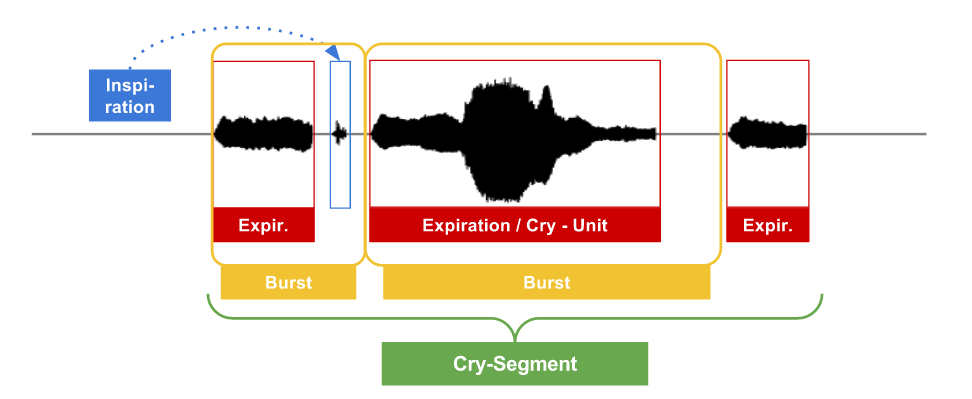
\includegraphics[width=0.7\textwidth]{bilder/cryVoc02.png}
	\caption{Veranschaulichung des Grundvokabulars}
	\label{img:cryVocabulary}
\end{figure}

Cry-Units werden von H Golub und M Corwin in eine der drei folgenen Kategorien eingeordnet, bezeichnet als \emph{Cry-Types}: \cite[S. 61 - 62]{cryModel}

\begin{itemize}
	 \item \textbf{Phonation} beschreibt eine Cry-Unit mit einer \glqq vollen Vibration der Stimmbänder\grqq{} und einer Grundfrequenz zwischen 250 und \SI{700}{\hertz}. Entspricht umgangssprachlich einem Weinen mit einem \glqq klaren, hörbaren Ton\grqq{}.
	 \item \textbf{Hyper-Phonation} beschreibt eine Cry-Unit mit einer \glqq falsetto-artigen Vibration der Stimmbänder\grqq{} mit einer Grundfrequenz zwischen 1000 und \SI{2000}{\hertz}. Entspricht umgangssprachlich einem Weinen mit einem \glqq sehr hohen, aber klar hörbaren Ton\grqq{}.
	 \item \textbf{Dysphonation} beschreibt eine Cry-Unit ohne klar feststellbare Tonhöhe, produziert durch Turbulenzen an den Stimmbändern. Entspricht umgangsprachlich dem \glqq Brüllen oder Krächzen\grqq{}.
\end{itemize}

Die folgenden weiteren Eigenschaften können für einzelne Cry-Units extrahiert werden:

\begin{itemize}
	\item \textbf{Duration:} Die zeitliche Dauer der Cry-Unit.
	\item \textbf{Duration of Inspiration: }Die zeitliche Dauer der Pause zwischen zwei Cry-Units.
	\item \textbf{Grundfrequenz:} Für eine Cry-Unit kann die durchschnittliche, die höchste und die niedrigste Grundfrequenz sowie die Varianz festgestellt werden.
	\item \textbf{Frequenz der Formanten:} Wie bei der Grundfrequenz kann der Durchschnitt, das Maximum, Minimum etc. für eine Cry-Unit berechnet werden.
	\item \textbf{Ratio2: } Verhältnis zwischen den Energien der Frequenzen unterhalb von \SI{2000}{\hertz} zu den Frequenzen oberhalb von \SI{2000}{\hertz}
	\item \textbf{Cry-Mode Changes:} Häufigkeit des Wechsels des Cry-Modes innerhalb einer Cry-Unit.
	\item \textbf{Amplitude:} Die Lautstärke der Cry-Unit, gemessen in Dezibel. \cite[S. 85]{parentalPerception} \cite[S. 156]{threeCryTypes}
\end{itemize}

Golub et al. haben weiterhin eine Reihe von Features vorgestellt, die das zeitliche Verhalten der Grundfrequenz und der harmonischen Obertöne innheralb einer Cry-Unit beschreiben. \cite[S. 73]{cryModel}

\begin{itemize}
\item \textbf{Pitch of Shift:} Grundfrequenz nach einem schnellen Anstieg zu Beginn der Cry-Unit
\item \textbf{Glide:} Kurzes, starkes ansteigen der Grundfrequenz
\item  \textbf{Glottal Roll:} Dysphonation, die häufig am Ende einer Cry-Unit nach einem Abfall der Grundfrequenz beobachtet wird.
\item  \textbf{Vibrato:} Mehr als vier starke Schwankungen der Grundfrequenz innerhalb einer Cry-Unit.
\item  \textbf{Melody-Type:} einer Cry-Unit. Meist: fallend, steigend/fallend, steigend, fallend/steigend, flach. 
\item  \textbf{Continuity:} Verhältnis zwischen stimmhaften und nicht-stimmhaften Bereichen der Cry-Unit
\item  \textbf{Double Harmonic Break:} Das Aufkommen einer zweiten Serie von harmonischen Obertönen zwischen den eigentlichen harmonischen Obertönen der Cry-Unit.
\item  \textbf{Biphonation:} Das Aufkommen einer zweiten Grundfrequenz mit eigenen harmonischen Obertönen zusätzlich zu der eigentlichen Grundfrequenz.
\item  \textbf{Noise Concentration:} Starke Energiespitzen zwischen 2000 und \SI{2300}{\hertz}.
\item  \textbf{Furcation:} Plötzliches Aufteilen der Grundfrequenz und harmonsichen Obertöne in mehrere, schwächere Obertöne.
\end{itemize}

Abbildung \ref{img:cryMelodies} visualsiert diese Grundfrequenz bezogenen Features in einem schematisch dargstellten Spektogramm.

\begin{figure}
	\centering
	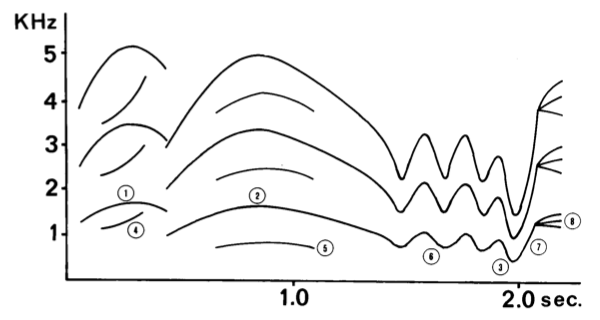
\includegraphics[width=0.7\textwidth]{bilder/melodyTypes.png}
	\caption{(1) Pitch of Shift (2) Maximale Grundfrequenz (3) Minimum der Grundfrequenz (4) Biphonation (5) Double Harmonic Break (6) Vibrato (7) Glide (8) Furcation \cite[S. 142]{signal}}
	\label{img:cryMelodies}
\end{figure}

Die folgende Features werden in Bezug auf das gesamte Cry-Segment, oder zumindest auf eine Menge aufeinander folgender Cry-Units berechnet:

\begin{itemize}
	\item \textbf{Cry Latence: } Zeit zwischen Stimulus, wie zum Beispiel einem Nadelstich, und erster Cry-Unit.
	\item \textbf{Utterances: } Anzahl der Cry-Units im Segment.
	\item \textbf{Short Utterances: } Anzahl stimmloser Cry-Units im Segment.
	\item .... und statistische Auswertungen bezüglich aller oben genannten Features, die sich auf eine Cry-Unit beziehen, wie beispielsweise der Durchschnitt aller durchschnittlichen Tonhöhen, Anzahl des Vorkommens bestimmter Melodiekonturen, Varianz der Länge der Cry-Units etc.\cite[S. 85]{parentalPerception}
\end{itemize}

Verschiedene Krankheitsbilder wurden in Zusammenhang mit dem vorkommen bestimmter Features des Cry-Segmentes gebracht. So wurde eine Korrelation zwischen dem Anstieg der durchschnittlichen Grundfrequenz, häufiger Biphonation und geringer Duration in Zusammenhang mit Gehirnschäden gebracht. Tendenziell niedrige Grundfrequenzen zeigen eine Korrelation mit Trisomie 13, 18 und 21\cite[S. 85]{parentalPerception}

\subsection{Diskussion}
\label{sec:cryDiscussion}

Bis heute bleibt die Analyse von kindlichen Lautäußerungen weitestgehend unstandartisiert \cite[S. 142]{signal}:
\begin{itemize}
\item Es gibt keine Einigung darüber, welche der zahlreichen vorgestellten Eigenschaften die wichtigsten sind. Beispielsweise konzentrierten sich Golub et al. \cite{cryModel} vermehrt auf die Erkennung von Mustern im Melodieverlauf, Zeskind et al. auf zeitliche Eigenschaften. \cite{rythmic}. Die Eigenschaft, die am häufigsten mit Schmerz, Krankheiten und sonstigen Abnormalitäten in Verbindung gebracht wird, ist eine abnormal hohe oder niedrige Tonhöhe. Bei einigen Features, die vor allem von Golub et al. verwendet wurden \cite{cryModel}, ist nicht einmal gesichert, ob es sich nicht doch um technische Artefakte der damals verwendeten Analogtechnik handelt. \cite[S. 84 - 85]{parentalPerception}
\item Zusammenhänge, die zwischen bestimmten Eigenschaften des Weinens und bestimmten Krankheitsbildern festgestellt wurden, haben häufig eine hohe Spezifität, aber niedrige Sensitivität. So wurde zum Beispiel festgestellt, dass Kinder, die am plötzlichen Kindstot verstarben, fast immer eine Erhöhung der Frequenz des ersten Formanten in Verbindung mit häufigen Cry-Mode-Changes zeigen. Viele Babys, die nicht am plötzlichen Kindstot versterben, zeigen jedoch die selben Merkmale.\cite[S. 85]{parentalPerception}
\item Selbst, wenn in verschiedenen Studien die selbe Eigenschaft verwendet wird, wie zum Beispiel die durchschnittliche Tonhöhe, ist nicht standardisiert, wie dieses exakt zu berechnen ist. Mit \glqq durchschnittliche Tonhöhe des Segmentes\grqq{} kann gemeint sein: (1) die Durchschnittliche Tonhöhe, errechnet aus den durchschnittlichen Tonhöhen der der Cry-Units (2) Die durchschnittliche Tonhöhe aller festgestellten Tonhöhen (3) die durchschnittliche Tonhöhe nur von Ausatmungslauten etc.
\item Golub et al. behaupten, bereits in den achziger Jahren ein System zur computergestützten und voll automatisierten Analyse von Cry-Segmenten implementiert zu haben. Das System nimmt (1.) eine Audioaufnahme, gespeichert auf einer Kasette an, (2.) berechnet Formanten, Grundfrequenz und Amplitude gegen die Zeit, (3.) samplt die Grundfrequenz-Kontur (4.) berechnet insgesamt 88 akkumulierte Features für das gesamte Segment und (5.) zieht Schlussfolgerungen aus den 88 Features, wie zum Beispiel die Diagnose einer bestimmten Krankheit.\cite[S. 75 - 76]{cryModel} Abseits der kurzen Erwähnung der Existenz dieser \grqq Mutter aller automatisierten Analysesysteme für das Weinen von Babys\grqq{} konnte der Autor dieser Arbeit keine Implementierungsdetails oder sonstige genaueren Ausführungen finden, welche für diese Arbeit von höchstem Interesse gewesen wären.
\end{itemize}


